\section{二足歩行ロボットの制御フロー}
\label{sec:control_flow}

本研究で用いる二足歩行ロボットの制御系は，計測情報に基づくフィードバック制御と歩行計画に基づく予測制御を組み合わせた階層的な構成をとっている．本節では，1 制御周期における制御フローの概要を，各処理段階に分けて説明する．制御フローの全体像を \cref{fig:control_flow} に示す．

\begin{figure}[htbp]
  \centering
  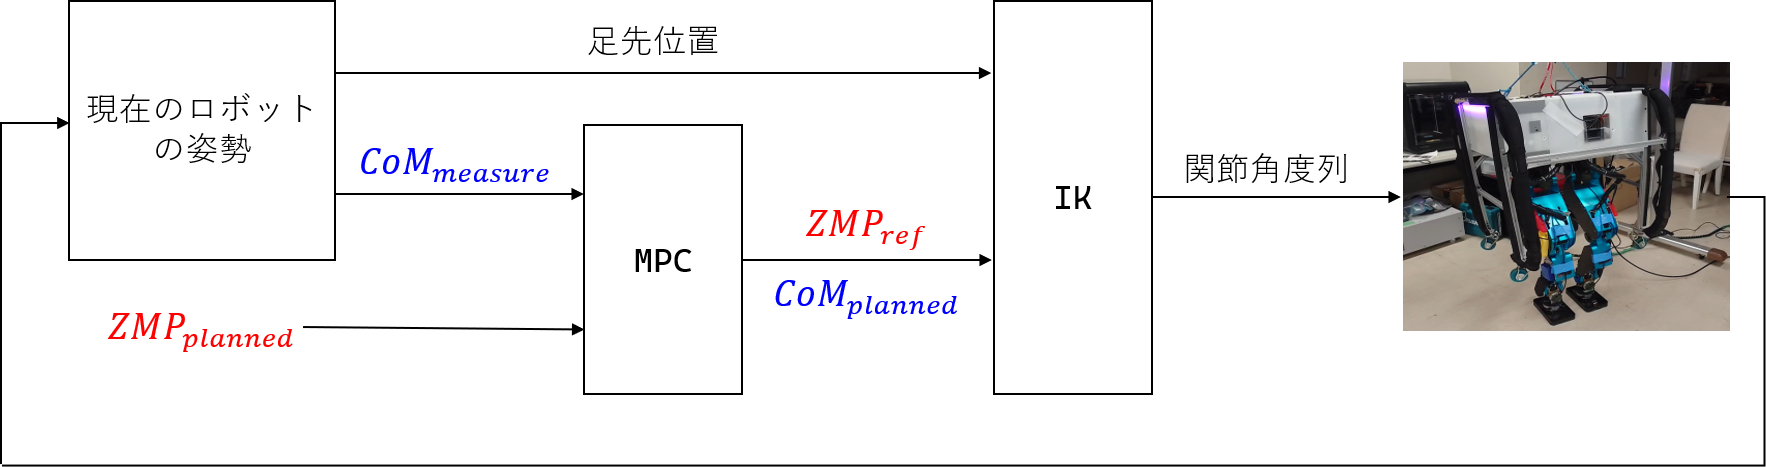
\includegraphics[width=1.0\linewidth]{images/control_flow.png}
  \caption{二足歩行ロボットの制御フロー}
  \label{fig:control_flow}
\end{figure}

\subsection{CoM 状態の計測と参照 ZMP 軌道}
\label{subsec:com_meas_zmp_planned}

各制御周期の開始時点において，ロボットの現在の CoM の計測値 $\mathrm{CoM}_{\mathrm{measure}}$ を取得する．この重心位置は，関節角度およびリンクモデルに基づいて算出された推定値であり，ロボットの実際の運動状態を反映した情報である．同時に，プログラム実行時にあらかじめ生成された ZMP の目標軌道 $\mathrm{ZMP}_{\mathrm{planned}}$ を参照する．$\mathrm{ZMP}_{\mathrm{planned}}$ は，歩行目標に基づいて生成された理想的な ZMP の時間推移を表しており，歩行中の安定性の基準となる．この段階では，$\mathrm{ZMP}_{\mathrm{planned}}$ はフィードフォワード的な情報として用いられる．

\subsection{モデル予測制御による目標 ZMP の生成}
\label{subsec:zmp_ref_generation}

次に，重心位置の計測値 $\mathrm{CoM}_{\mathrm{meas}}$ と目標軌道 $\mathrm{ZMP}_{\mathrm{planned}}$ を入力として，モデル予測制御（Model Predictive Control: MPC）を適用する．MPC では，ロボットの動力学モデルを用いて将来の状態を予測し，歩行の安定性を満たすように最適化を行うことで，次の制御周期における目標軌道$\mathrm{ZMP}_{\mathrm{ref}}$ を生成する．この処理により，歩行計画で与えられた理想的な ZMP 軌道と実際のロボット状態との偏差が補償され，外乱やモデル誤差に対してロバストな ZMP 指令が得られる．生成された $\mathrm{ZMP}_{\mathrm{ref}}$ は，後段の重心目標生成および全身運動生成の基準となる．

\subsection{目標 ZMP に基づく重心目標軌道の生成}
\label{subsec:com_planned_generation}

生成された $\mathrm{ZMP}_{\mathrm{ref}}$ を基に，次に重心の目標軌道 $\mathrm{CoM}_{\mathrm{planned}}$ を計算する．この段階では，ZMP と重心運動の関係に基づくモデルを用い，$\mathrm{ZMP}_{\mathrm{ref}}$ を実現するために必要な重心位置およびその時間変化を決定する．$\mathrm{CoM}_{\mathrm{planned}}$ は，歩行中の安定性を直接左右する重要な目標量であり，特に支持脚切替時や外乱が加わった場合において，ロボットの転倒を防ぐための役割を担う．この重心目標は，次段階の全身逆運動学における拘束条件として用いられる．

\subsection{全身逆運動学による関節角度の生成}
\label{subsec:whole_body_ik}

最後に，現在の足先位置，重心の目標軌道 $\mathrm{CoM}_{\mathrm{planned}}$，および目標ZMP軌道 $\mathrm{ZMP}_{\mathrm{ref}}$ を拘束条件として，全身逆運動学（Whole-body Inverse Kinematics: IK）を解く．全身 IK では，足先の接地条件を満たしつつ，重心位置および ZMP 目標を実現するように，ロボット全体の関節角度が一貫した形で決定される．この結果として，各関節に対する目標関節角度列が生成され，これが下位の関節制御系に入力されることで，ロボットの運動が実現される．以上の処理を各制御周期で繰り返すことで，安定した二足歩行が実現される．
